\documentclass[12pt,a4paper]{article}
\usepackage{geometry}
\usepackage{slashbox}
\geometry{
	a4paper,
	total={170mm,257mm},
	left=20mm,
	right=20mm,
	top=20mm,
	bottom=20mm
}
\usepackage{graphicx}
\usepackage{pdfpages}
\usepackage{placeins}
\usepackage{float}

\usepackage{polski}
\usepackage[utf8]{inputenc}

\begin{document}
	
	\begin{titlepage}
		\newgeometry{top=5.5cm, bottom=3cm}
		
		\centering
		{\huge\bfseries Logika układów cyfrowych lab.\par}
		
		\vspace{0.5cm}
		Prowadzący: Mgr inż. Antoni Sterna (E02-38m, wtorek 17:05) \\
	
		\vspace{1.1cm}
		{\Large sprawozdanie 8 - 2017.12.04\par}
		\vfill
		
		{\large\bfseries Jakub Dorda 235013\par}
		{\large\bfseries Marcin Kotas 235098\par}
		
		\vspace{1cm}
		\today \\ \LaTeX
		
		\restoregeometry
	\end{titlepage}

	\newgeometry{top=1.5cm, bottom=1.5cm, left=20mm, right=20mm}

	\section{Wprowadzenie/cel ćwiczeń}
	
		Celem ćwiczenia było zapoznanie się z działaniem automatów niedeterministycznych.
		W tym celu należało przeanalizować schemat w instrukcji odpowiadający automatowi NFA dla wyrażenia 0*1*2.
		Następnym zadaniem było przygotowanie modyfikacji automatu tak, aby odpowiadał on wyrażeniu 0*(1+2)*.
		
	\section{Opis działania:}

			Wszystkie wejścia automatu powinny być wejściami impulsowymi (poza wejściem odpowiadającym przejściu pustemu \(\epsilon\)).
			Z uwagi na to, że w zestawach UNILOG dostępne są tylko 3 wejścia impulsowe, przeznaczone one zostały na wejścia RESET, START, READ.
			Pozostałe wejścia podłączone zostały do zwykłych wejść.

		\subsection{RESET:}
			Wejście RESET powoduje wyzerowanie wszystkich przerzutników.
			Poszczególne przerzutniki odpowiadające konkretnym stanom automatu mogą zostać również wyzerowane w wyniku działania automatu.
			Przerzutnik pierwszy może zostać wyzerowany w wyniku podania na wejście automatu cyfry 1 lub 2, oraz w wyniku wciśnięcia przycisku READ.
			Podobnie przerzutnik drugi wyzerowany zostanie przy aktywowaniu przerzutnika trzeciego, a więc podaniu cyfry 2 oraz wciśnięciu READ.
			Wszystkie stany wyzerowane zostaną również, gdy podana zostanie niedozwolona cyfra - np. 1 po 2, lub 0 po 1 lub 2.

		\subsection{START:}
			Wejście START wprowadza automat w początkowy stan, należy go użyć po wciśnięciu przycisku RESET. 

		\subsection{READ:}
			Wejście READ sprawdza, czy do automatu wprowadzono poprawne słowo.
			Jeśli któryś ze stanów automatu był aktywny to oznacza, że do tego momentu wprowadzone zostały poprawne cyfry.
			W takim wypadku wciśnięcie READ powoduje uaktywnienie stanu końcowego oraz zmianę wyjścia na 1.
			Jeśli w momencie wciśnięcia READ żaden ze stanów nie był aktywny - wprowadzono złe słowo, to wyjście się nie zmienia.

		\subsection{Wejścia SET przerzutników}
			Na wejścia SET przerzutników podłączony jest zestaw bramek złożony z 2 bramek AND oraz jednej NOR.
			Mają one za zadanie sprawdzać poszczególne warunki, dla których uaktywni się poszczególny stan.
			Np. drugi stan końcowy uaktywni się w następujących przypadkach: jeśli wprowadzona została cyfra 2 i jednocześnie aktywny był którykolwiek ze stanów,
			oraz jeśli aktywowane zostało wejście READ i którykolwiek ze stanów był aktywny.

		\vspace{1.5cm}
		\begin{center}
			%\makebox[\textwidth]{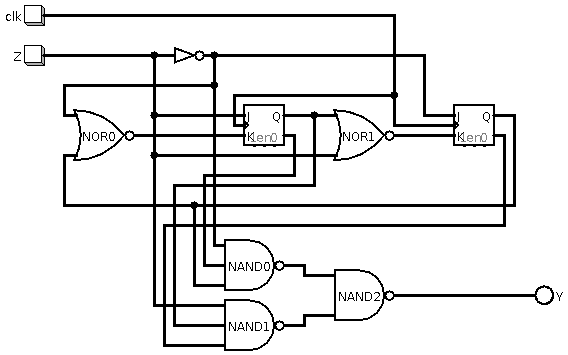
\includegraphics[width=\paperwidth - 40mm]{schem/circuit1.png}}
			Schemat 1 - analizator ciągu par w wersji Mealy
		\end{center}

	\section{Wnioski/podsumowanie}
	
			W celu sprawdzenia poprawności działania komparatora należało przeprowadzić testy dla wszystkich możliwych kombinacji wejść oraz stanów. W czasie testowania układu okazało się, że typ zbocza sygnału reset może mieć
			wpływ na poprawne zachowanie automatów ze względu na budowę wewnętrzną przerzutników. 
	
\end{document}